\chapter{Future Steps}

\section{ROS Navigation Stack}

\subsection{ros\_controller}
\begin{figure}[h]
	\caption{ROS control overview \cite{fig_ros_control}}
	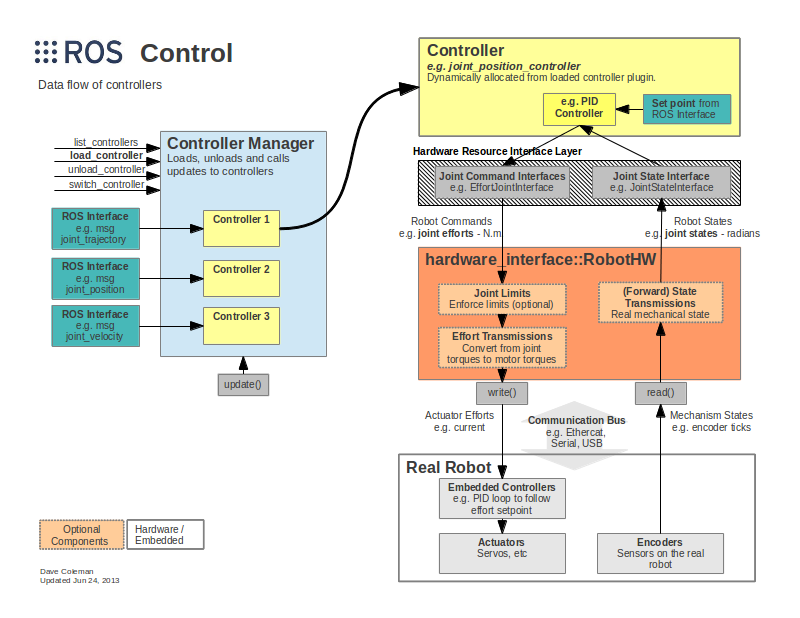
\includegraphics[]{gazebo_ros_control}
	\label{fig:ros_controller}
\end{figure}

\section{Field Test scenario}

\subsection{GPS Waypoints}
GPS markers form a linearized path
travel in a straight line from one GPS node to another
%https://www.google.com/maps/d/edit?mid=1wKgTvF7i7Xdpi42cw1ffAOrGDVw&ll=27.38460862376806%2C-82.56151826455687&z=17


\section{Project Limitations}
how this project is limited

introduction of a camera, but attaching a webcam directly to the chassis of the robot would be troublesome to work with, sense there would be no shock absorption and the video frames would wobble.

Integration of GPS data into position estimate causes discrete jumps, may make it unsuitable for use in the navigation stack. Solution: ditch GPS, use range data from ultrasonic sensor with amcl


\section{Conclusion}
